\documentclass[../ZF_Wing.tex]{subfiles}

\begin{document}

\textbf{Ziel:} Wettbewerbsfähigkeit des Betriebs.\\
\textbf{Gründe:} liegen in der Dynamik des Marktes.\\
\begin{itemize}
	\item Steigerung der Produktivität
	\item Globalisierung
	\item Kostenreduzierung
	\item Erhöhung der Flexibilität
	\item Senkung der Durchlaufzeit
	\item Kundenorientierung
\end{itemize}
\textbf{Definition:} Zahlungsreihe, die i.d.R mit einer sicheren Auszahlung beginnt, 
auf die zu späteren Zeitpunkten unsichere Einnahmen folgen. Wird dirket aus der Strategie abgeleitet.

\subsection{Cashflow}
\textbf{Auszahlungen (Aufwand):}
\begin{itemize}
	\item Erstinvestition / einmalige Zahlung / Anschaffung
	\item Anlaufkosten / Inbetriebnahmekosten
	\item Schulungskosten
	\item Lfd. Kosten
\end{itemize}
\textbf{Einzahlungen (Erträge):}
\begin{itemize}
	\item Absatzsteigerung
	\item Einsparungen von Ressourcen
	\item Preiserhöhung
	\item Erweiterung des Produktspektrums
\end{itemize}


\subsection{Kategorien von Investitionsprojekten}
\begin{itemize}
	\item Sachvermögen
	\item Finanzlangen
	\item Immaterielles Vermögen
\end{itemize}

\subsection{Investitionsgründe}
\begin{itemize}
	\item Normativ
	\item Strategisch
	\begin{itemize}
		\item Technologiewechsel
		\item Make-or-Buy
	\end{itemize}
\end{itemize}

\subsection{Methoden Investitionsrechnung}
\begin{itemize}
	\item Statische Methoden
	\begin{itemize}
		\item Kostenvergleichsrechnung
		\item Gewinnvergleichsrechnung
		\item Rentabilitätsrechnung (ROI)
		\item Amortisationsrechnung (Payback)
	\end{itemize}
	\item Dynamische Methoden
	\begin{itemize}
		\item Barwertmethode (NPV / DCF)
	\end{itemize}
\end{itemize}

\subsubsection{Kostenvergleichmethode}
\textbf{\textcolor{purple}{Variable Kosten}} $ = Jaehrliche Betriebskosten + Materialkosten$\\
\textbf{\textcolor{purple}{Fixe Kosten}} $ = Kalkulatorische Abschreibungen + Kalkulatorische Zinsen$\\
\textbf{\textcolor{brown}{Gesamtkosten}} = \textbf{\textcolor{purple}{Variable Kosten}}+ \textbf{\textcolor{purple}{Fixe Kosten}}

\subsubsection{Gewinnvergleichsmethode}
\textbf{\textcolor{green}{Jährlicher Gewinn}} = Jährlicher Nettoerlös - Variable Kosten - Fixe Kosten\\



\subsubsection{Rentibilitätsvergleich}
\textbf{\textcolor{orange}{Rentabilität}} $= \dfrac{Reingewinn + Kalk. Zinsen}{eing.Kapital}*100$ 

\subsubsection{Payback-Frist (Amortisation)}
Je früher desto besser.\\
\textbf{\textcolor{magenta}{Payback-Frist}} $= \dfrac{Kapitaleinsatz}{Jaehrl.Cashflow}$ \\\\
\textbf{\textcolor{magenta}{Indirekter Cashflow}} $= Reingewinn + Abschreibungen + FK-Zinsen$\\ 
\textbf{\textcolor{magenta}{Direkter Cashflow}} $= Jaehrl.Nettoerloes -(jaehr.Betriebs$- und $Materialkosten)$\\ 

\subsection{Dynamische Investiotionsrechnung}
\textbf{Aufzinsung}\\
$K_{0} * (1 + i)^{n} = K_{n}$\\\\
\textbf{Abzinsung}\\
$K_{n} * 1+(1 + i)^{n} = K_{0}$\\\\
\begin{figure}[H]
\centering
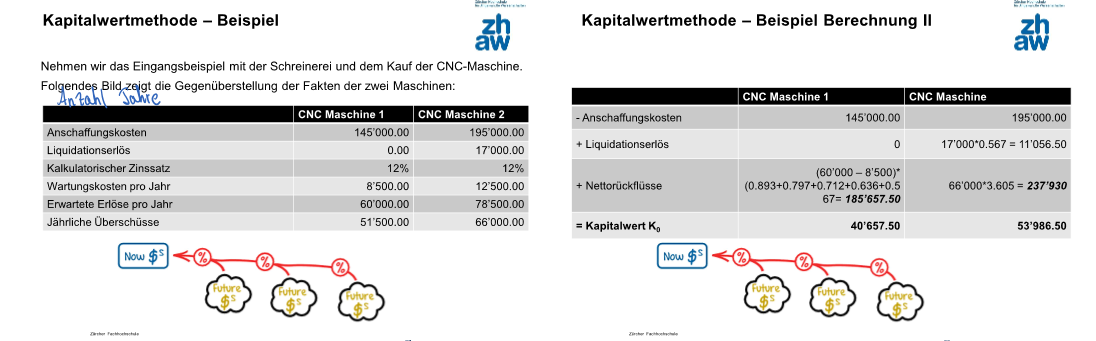
\includegraphics[width=0.3\textwidth]{Resources/Image/Kapitalwertmethode.png}
\caption{\label{fig:Kapitalwertmethode}Kapitalwertmethode.}
\end{figure}
\begin{figure}[H]
\centering
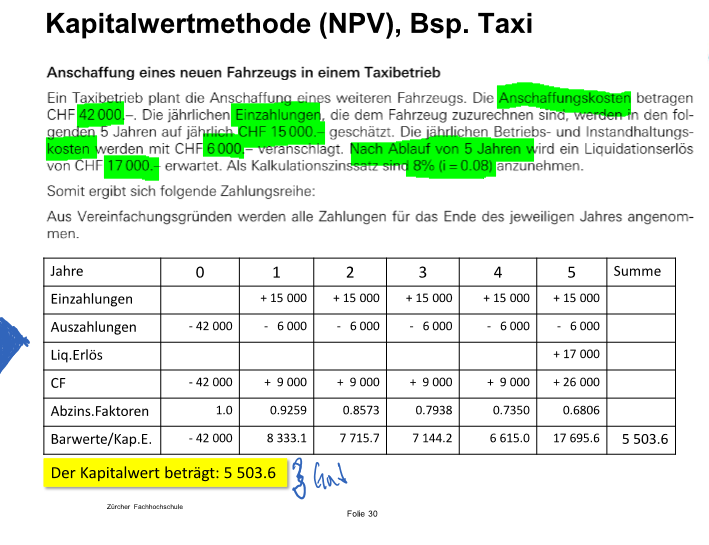
\includegraphics[width=0.3\textwidth]{Resources/Image/Kapitalwertmethode2.png}
\caption{\label{fig:Kapitalwertmethode2}Kapitalwertmethode2.}
\end{figure}
Einfluss positiver NPV auf den Wert eines Unternehmens:\\
\begin{itemize}
	\item Erhöht finaziellen Wert des Unternehmens
	\item Kosten für Investition sind gedeckt und resultieren Nettoeinnahmen nach Ablauf der Laufzeit.
	\item Unternehmenswert steigt genau um Nettoeinnahmen
\end{itemize}















\end{document}